\setlength{\tabcolsep}{6pt}
\renewcommand{\arraystretch}{1.5}
\begin{figure}[!t]
    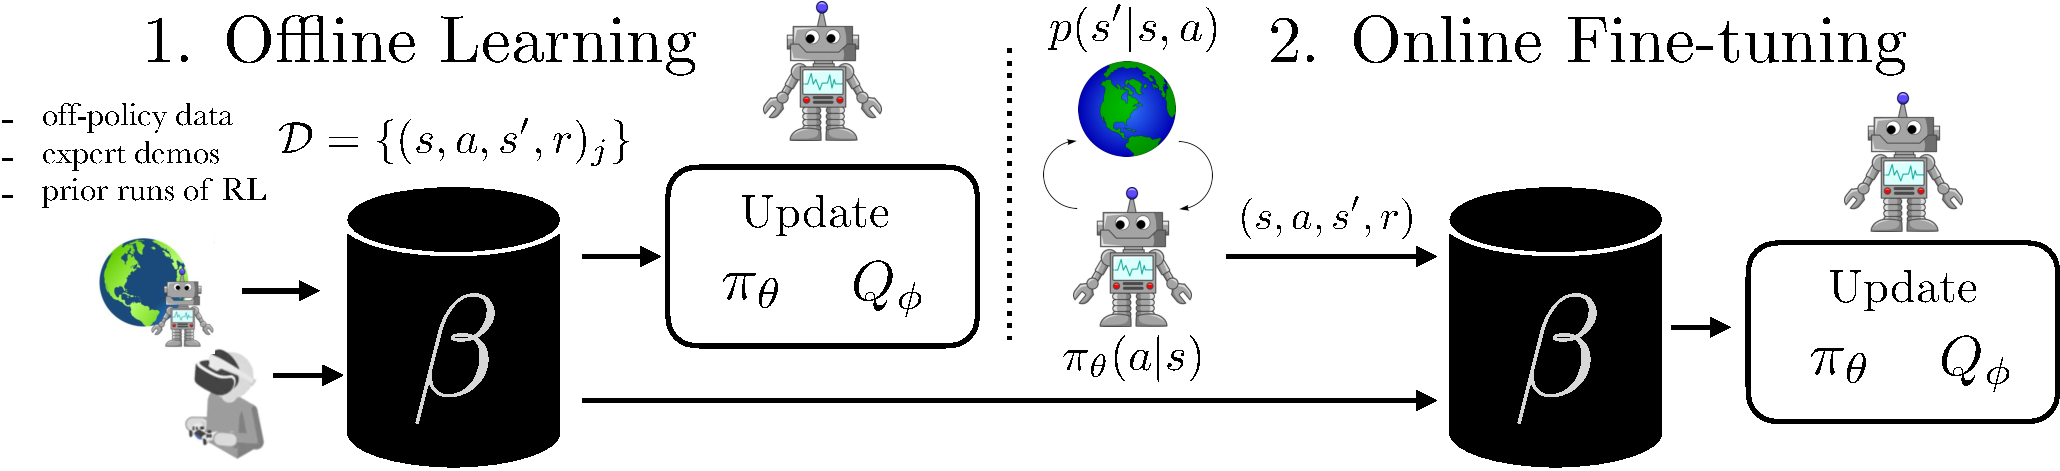
\includegraphics[width=0.99\textwidth]{awac/figures/fig1v2-crop.pdf}
    \caption{
    % \small{
    % \footnotesize{
    We study learning policies by offline learning on a prior dataset $\mathcal{D}$ and then fine-tuning with online interaction. The prior data could be obtained via prior runs of RL, expert demonstrations, or any other source of transitions. Our method, advantage weighted actor critic (AWAC) is able to learn effectively from offline data and fine-tune in order to reach expert-level performance after collecting a limited amount of interaction data.
    Videos and data are available at \projectpage
    % }
    % Videos and code are available at \href{https://awacrl.github.io/}{\textit{awacrl.github.io}}
    % }
    %\vspace{-0.3cm}
    }
    \label{fig:figure1}
\end{figure}